\documentclass[sigplan,screen]{../../acmart}

\AtBeginDocument{%
  \providecommand\BibTeX{{Bib\TeX}}%
}

\setcopyright{none}
\settopmatter{printacmref=false, printccs=false}
\copyrightyear{2026}
\acmYear{2026}
\acmDOI{}
\acmConference[Draft]{Draft manuscript}{June 2026}{Busan, Republic of Korea}
\acmISBN{}

\usepackage{kotex}
\usepackage{amsmath}
\usepackage{array}
\usepackage{booktabs}
\usepackage{bbm}
\usepackage{siunitx}
\graphicspath{{figures/}{../../figures/}}
\newcommand{\Ind}{\mathbbm{1}}
\newcolumntype{L}[1]{>{\raggedright\arraybackslash}p{#1}}
\emergencystretch=2em

\title{PUBG 텔레메트리의 시공간 데이터베이스 표현과 페이즈별 생존 예측}

\author{Seong Eun BAEK}
\email{todtjddms104204@pusan.ac.kr}
\affiliation{%
  \institution{Pusan National University}
  \city{Busan}
  \country{Republic of Korea}
}

\author{Joonho KWON}
\email{jhkwon@pusan.ac.kr}
\affiliation{%
  \institution{Pusan National University}
  \city{Busan}
  \country{Republic of Korea}
}

\renewcommand{\shortauthors}{Baek and Kwon}

\begin{document}

\begin{abstract}
배틀로얄 장르의 게임에서 최종 순위는 경기 종료 후 기록되는 단일 결과값이지만,
실제로는 각 팀이 시간에 따라 변화하는 공간, 자원, 교전 사건, 생존 상태 속에서
여러 페이즈를 통과하거나 탈락하는 과정의 결과다. 이 논문은 PUBG: Battlegrounds
스쿼드 매치의 공식 텔레메트리(telemetry)를 경기 후 집계 행으로 보지 않고,
시공간 데이터베이스 표현으로 다시 구성한다. 스쿼드 팀은 이동 객체, 안전구역과
블루존은 시간변화 영역, 피해 사건, 기절 사건, 처치 사건, 탈락 사건은 시공간
사건으로 둔다. 이를 페이즈별 위험집합(risk set)과 10초 간격 팀 상태 관측값으로
변환한다.

최종 순위 예측은 이 표현 위에서 다음 페이즈 탈락 위험도(hazard) 예측 문제로
바뀐다. 9개 맵/플레이 모드 조건의 2,500개 스쿼드 매치로 초기 비교 실험을 수행한
결과, 가장 안정적인 신호는 페이즈별로 갱신되는 팀 생존 여력이었다. 이는 전투 생존
게임에서 평균 체력, 최소 체력, 생존 인원, 차량 이용 여부 같은 직접 상태 변수가
강하게 작동한 결과로 해석해야 한다. 더 중요한 비교는 직접 생존 상태를 제외한
조건에서도 이동 이력이 의미를 갖는지이다. 이동 이력
조건은 팀 중심 좌표와 속도의 10초 이력만으로 다음 페이즈 탈락을 예측했으며, 페이즈
종료 시점의 단일 상태만 사용하는 기준모델(baseline)보다 낮은 손실을 보였다. 반대로
안전구역 맥락은 단독 조건과 이동 이력과의 단순 결합 조건에서 뚜렷한 개선을 만들지
못했다.

이 결과를 안전구역이 불필요하다는 뜻으로 읽기는 어렵다. 더 정확한 해석은 현재
구성에서 먼저 보존되어야 할 정보가 팀의 생존 상태와 이동 이력이며, 안전구역은
독립 특징으로 붙이는 방식보다 이동 이력과 생존 상태의 의미를 조건화하는 표현으로
다시 설계되어야 한다는 것이다.
\end{abstract}

\keywords{배틀로얄 게임, PUBG 텔레메트리, 시공간 데이터베이스, 페이즈별 생존 예측, 탈락 위험}
\maketitle

\section{서론 및 문제 정의}
\label{sec:problem}

PUBG: Battlegrounds와 같은 배틀로얄 장르의 게임에서 한 팀의 최종 순위는 경기
종료 시점에 부여되는 값이지만, 그 순위는 경기 도중 반복되는 생존과 탈락의
순서에 의해 결정된다. 팀은 넓은 맵에 진입해 자원을 확보하고, 다른 팀과의 접촉을
피하거나 감수하며, 점차 축소되는 안전구역 안에서 다음 페이즈를 버텨야 한다.
같은 이동 거리라도 초반의 이동과 후반의 이동은 다른 의미를 갖는다. 초반의 긴
이동은 자원 확보나 위치 선점을 위한 선택일 수 있지만, 후반의 짧은 이동은 블루존
피해, 남은 팀의 밀도, 체력 상태와 결합되어 곧바로 탈락 위험으로 이어질 수 있다.
따라서 PUBG의 순위를 경기 종료 후의 단일 행으로만 다루면, 어떤 팀이 어느
시점에서 위험해졌고 그 위험이 어떤 상태와 이동 이력에서 발생했는지를 잃게 된다.

기존 PUBG 순위 예측 연구는 최종 순위가 데이터로 예측 가능하다는 점을 보여주었다
\cite{kagglePubgFinishPlacement,rokad2019pubgPlacement,sen2021pubgFinalRank,lee2025pubgRank}.
그러나 페이즈별 생존을 묻기 시작하면 문제의 단위가 달라진다. 필요한 것은
``이 팀은 최종적으로 몇 등인가''가 아니라, ``이 팀은 지금까지 관측된 정보만으로
다음 페이즈를 버틸 수 있는가''이다. 이 차이를 다루려면 먼저 로그를 자르는 방식부터
바뀌어야 한다. PUBG 텔레메트리를 경기 후 집계 행이 아니라 이동 객체, 시간변화
영역, 시공간 사건, 페이즈별 위험집합으로 재구성하고, 그 표현이 다음
페이즈의 탈락 위험 예측을 어떻게 가능하게 하는지 확인한다.

본 논문에서 말하는 배틀로얄 장르의 매치는 네 가지 구조를 갖는 게임 플레이
단위로 정의한다. 첫째, 다수의 플레이어 또는 팀이 하나의 경기장 또는 맵에 동시에
배치된다. 둘째, 플레이 가능한 영역은 시간에 따라 축소되고, 그 밖의 영역은
피해를 주는 위험 구역으로 작동한다. 셋째, 팀은 자원, 이동성, 체력, 교전 노출을
관리하며 다음 페이즈까지 생존해야 한다. 넷째, 최종 순위는 각 팀의 탈락 시점에
의해 정해진다. 이 구조를 일반화하면 하나의 매치 \(M\)은 다음과 같이 표현할 수
있다.
\[
M=\langle A,\Omega,T,Z_{1:T},R_{1:T},C_{1:T},S_{1:T},Y\rangle .
\]
여기서 \(A\)는 생존 주체인 플레이어 또는 팀, \(\Omega\)는 경기장 또는 맵,
\(T\)는 매치 시간 또는 페이즈 순서, \(Z_{1:T}\)는 시간에 따라 변하는 안전구역과
위험 구역이다. \(R_{1:T}\)는 아이템, 차량, 회복 수단 같은 자원 상태이고,
\(C_{1:T}\)는 피해, 기절, 처치, 조우 같은 교전 사건이다. \(S_{1:T}\)는 각 주체의
위치와 생존 상태 변화이며, \(Y\)는 탈락 시점과 최종 순위이다. 이 표현에서 순위는
별도의 정적 라벨이 아니라, 페이즈별 위험을 통과하거나 통과하지 못한 순서의 누적
결과다.

그림~\ref{fig:team-phase-st-example}은 이 구조를 실제 PUBG 맵 위에서 보여준다.
한 팀은 낙하지점에서 출발해 페이즈마다 다른 이동 궤적을 남기고, 안전구역 경계가
이동할수록 같은 좌표도 다른 의미를 갖는다. 이 그림에서 중요한 것은 경로의 모양
자체가 아니다. 경로가 어느 페이즈의 어떤 안전구역 안에서, 어떤 탈락 시점으로
이어졌는지가 생존 문제의 단위가 된다.

\begin{figure}[t]
\centering
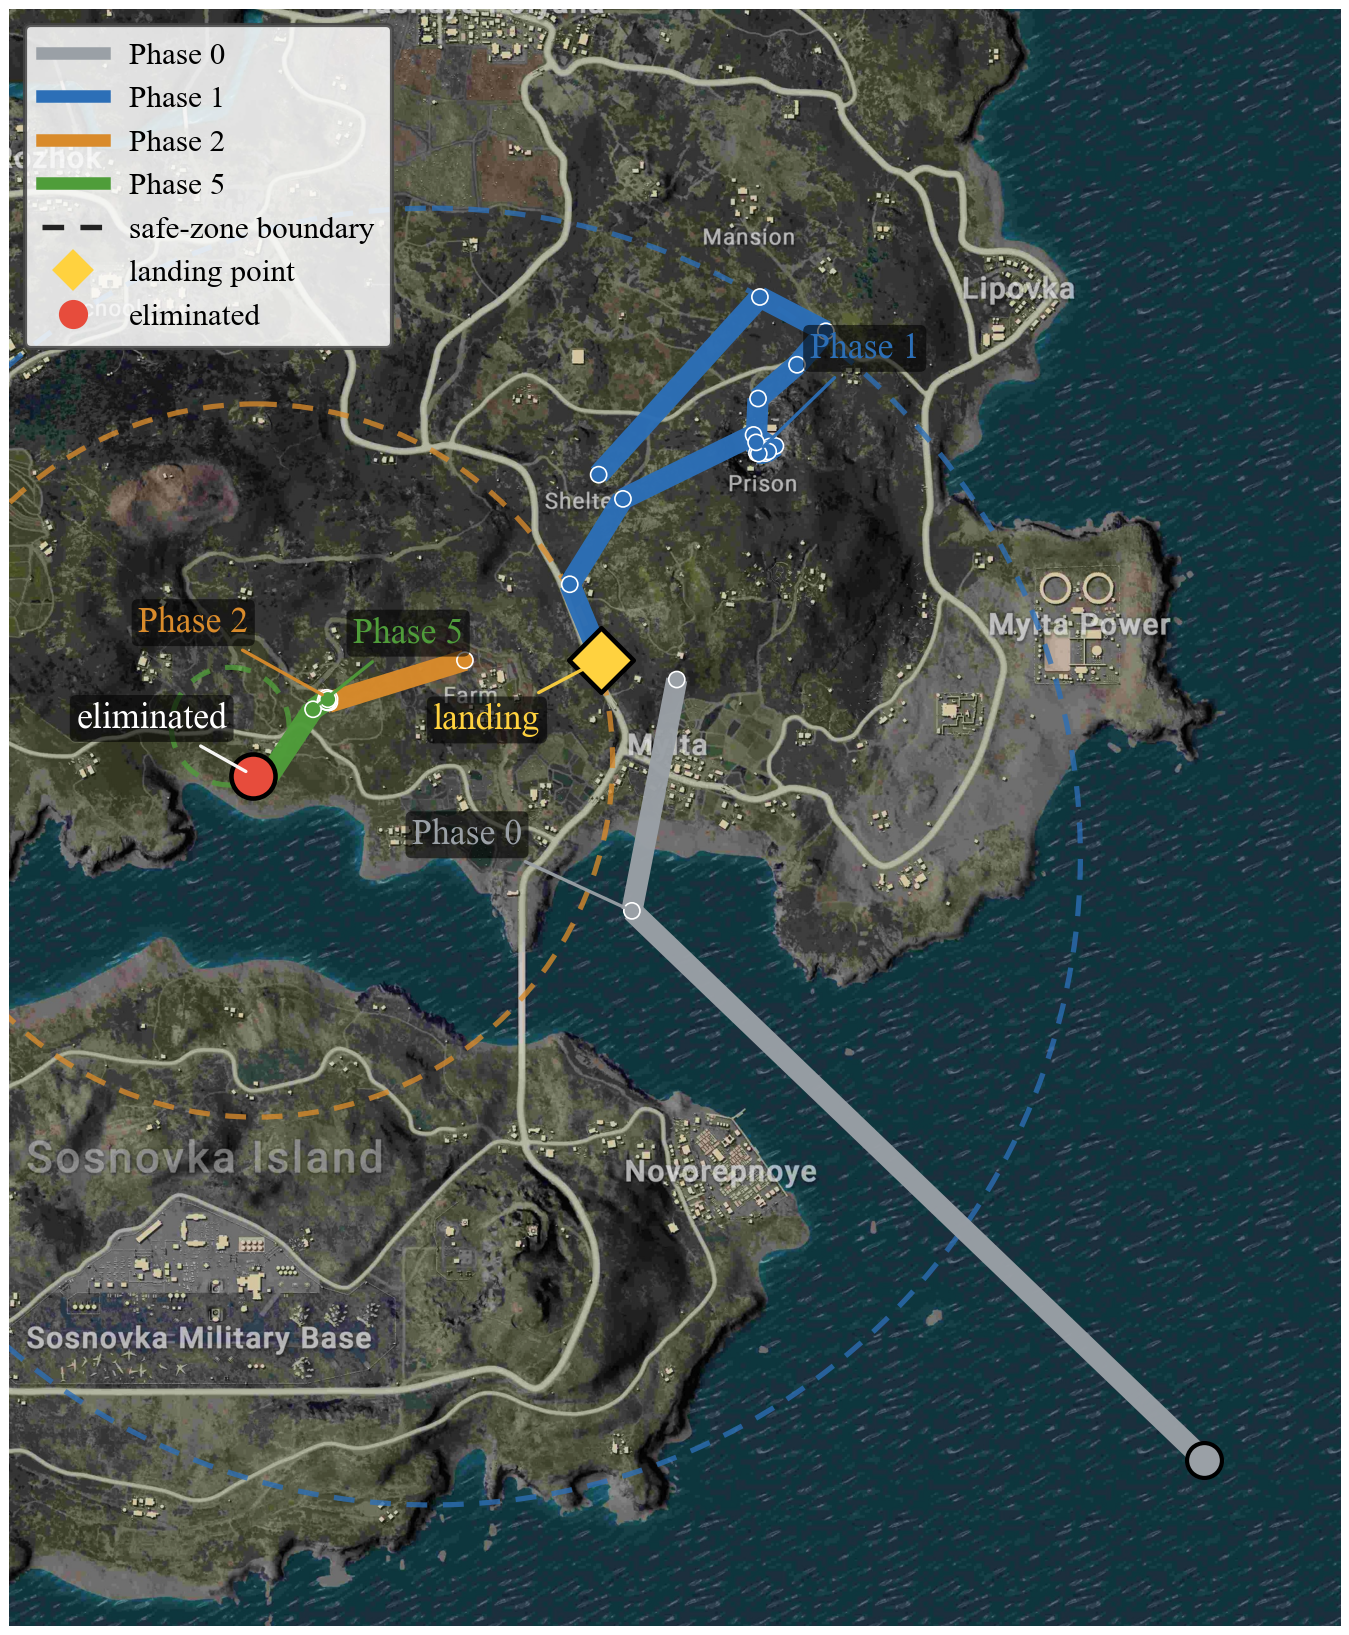
\includegraphics[width=\linewidth]{team_phase_feature_example.png}
\caption{PUBG 텔레메트리를 페이즈별 생존 이력으로 본 예. Erangel 맵 위에 한
팀의 이동 궤적, 페이즈별 안전구역 경계, 낙하지점, 탈락 지점을 함께 표시했다.}
\Description{Erangel 맵 위에 한 팀의 이동 경로와 여러 페이즈의 안전구역 경계,
낙하지점, 탈락 지점을 겹쳐 표시한 시공간 생존 이력 예시.}
\label{fig:team-phase-st-example}
\end{figure}

PUBG: Battlegrounds는 이러한 구조를 관측하기에 적합한 사례이다. 한 매치는 최대
100명의 플레이어를 큰 맵에 배치하고, 안전구역 축소와 블루존 피해 속에서 마지막
생존자를 가린다 \cite{pubgGameInfo}. 공식 개발자 API는 시간순 텔레메트리, 위치
기록, 구역 상태, 교전 사건, 탈락 사건을 제공한다
\cite{pubgDeveloperPortal,pubgTelemetryGuide,pubgTelemetryEvents,pubgTelemetryObjects}.
물론 이 자료가 지형, 엄폐, 시야, 숙련도, 팀 의사소통을 모두 담지는 못한다.
그럼에도 각 팀이 어디에 있었고, 어떤 자원과 체력 상태로 움직였고, 어떤 접촉이나
구역 압력 아래에서 탈락했는지는 재구성할 수 있다.

이 논문의 초점은 특정 예측 모델의 최종 성능 경쟁이 아니다. 먼저 PUBG 텔레메트리를
시공간 데이터베이스 관점에서 어떻게 잘라야 페이즈별 생존 문제가 되는지 묻고, 그
표현이 예측에서 어느 정도 작동하는지 확인한다. 연구 질문은 다음과 같이 좁힌다.

\noindent\textbf{RQ1.} PUBG 스쿼드 매치의 공식 텔레메트리는 이동 객체, 시간변화
영역, 시공간 사건, 페이즈별 위험집합으로 구성된 시공간 데이터베이스
표현으로 재구성될 수 있는가?

\noindent\textbf{RQ2.} 최종 순위 또는 페이즈 종료 시점의 단일 상태로 압축된
표현보다, 페이즈별 시공간 이력을 보존한 표현이 다음 페이즈의 탈락 위험 예측에 더
유용한가?

\noindent\textbf{RQ3.} 직접 생존 상태 변수와 이동 이력, 안전구역 맥락을 분해했을 때
각 구성요소는 다음 페이즈 생존 예측에서 어떤 역할을 하는가?

이 질문들은 특정 모델이나 구성요소가 반드시 우수해야 한다는 가정에서 출발하지
않는다. 중요한 것은 PUBG 스쿼드 매치를 시공간 데이터베이스로 재구성했을 때 생존
예측 문제가 어떻게 정의되고, 어떤 구성요소가 먼저 작동하며, 어떤 구성요소는 더
정교한 표현 설계를 요구하는지 분리하는 것이다.

\section{관련 연구}
\label{sec:related-work}

\subsection{최종 순위 예측에서 페이즈별 생존 예측으로}

PUBG 예측 연구의 출발점은 경기 종료 후의 최종 순위였다. Kaggle의 PUBG Finish
Placement Prediction 데이터셋은 처치 수, 피해량, 이동 거리, 회복 아이템 사용량,
매치 유형 같은 경기 후 집계값으로 \texttt{winPlacePerc}를 예측한다
\cite{kagglePubgFinishPlacement}. Rokad 등, Sen 등, Lee와 Lee의 연구도 PUBG의
최종 순위와 관련된 변수와 예측 가능성을 다루었다
\cite{rokad2019pubgPlacement,sen2021pubgFinalRank,lee2025pubgRank}. 이 연구들은
PUBG 순위가 로그 기반 변수로 예측 가능하다는 점을 보여주지만, 대부분의 접근은
매치를 이미 끝난 하나의 기록으로 압축한다. 페이즈별 생존 문제에서는 이 압축이
강한 단순화가 된다. 같은 총 피해량이나 이동 거리도 전혀 다른 노출 이력에서 나올
수 있기 때문이다.

Sagong 등의 연구는 이러한 압축을 풀기 시작한 중요한 선행 작업이다
\cite{sagong2025hunterCamper}. 이들은 PUBG 로그를 페이즈별로 나누고, 공격성과
활동성을 나타내는 점수로 Hunter, Sniper, Traveler, Camper 같은 전략 유형을
구성한 뒤 다음 페이즈 생존과 승리를 예측했다. 이 논문은 그 문제의식을 이어받되,
전략 유형보다 앞선 표현 단위로 돌아간다. 팀의 상태, 이동, 안전구역 맥락을 어떤
절단 시점에서 관측해야 다음 페이즈의 탈락 위험 문제가 되는지를 묻는다.

\subsection{텔레메트리, 이동 이력, 동적 공간 맥락}

게임 텔레메트리 연구는 행동 로그가 단순 이벤트 기록을 넘어 플레이어 행동을
정량화하는 자료가 될 수 있음을 보여준다. Drachen 등은 행동 로그 기반 군집화와
프로파일 해석을 다루었고 \cite{drachen2014behavioralTelemetry}, Bunian 등은 행동의
순서가 집계 횟수보다 플레이어 차이를 더 잘 드러낼 수 있음을 보였다
\cite{bunian2018hmmGameBehavior}. 배틀로얄 장르의 게임에서는 이 순서성이 특히
중요하다. 예측 시점 이후의 피해량, 위치, 탈락 사건이 입력에 섞이면 모델은 생존을
예측하는 것이 아니라 이미 일어난 결과를 확인하게 된다.

이동 궤적 분석은 움직이는 대상을 시간순 공간 표본으로 다루는 언어를 제공한다
\cite{wang2020trajectorySurvey}. 팀 스포츠의 시공간 분석도 개별 선수의 행 단위
통계만으로는 결과를 충분히 설명하기 어렵고, 위치와 상호작용을 함께 보아야 함을
보여준다 \cite{gudmundsson2016teamSportsSurvey}. PUBG 스쿼드 매치 역시 하나의
팀이 함께 움직이며 생존하지만, 여기에 추가 조건이 있다. 팀이 움직이는 공간 자체가
페이즈마다 축소된다. 여기서 이를 생물학적 habitat으로 주장하려는 것은 아니다. 중요한
것은 플레이 가능 영역이 줄어들고, 위치의 위험도가 페이즈에 따라 바뀌며, 남은
팀들이 점점 좁은 공간에 모인다는 구조다 \cite{fahrig2003fragmentation,nathan2008movement}.

\subsection{페이즈별 생존 모델링}

마지막으로 생존분석은 이 문제를 최종 라벨 분류가 아니라 구간별 위험으로 읽게 해
준다. 이산 시간 사건사 모델은 각 구간에서 누가 아직 위험집합에 남아 있고, 그
구간에 사건이 발생했는지를 정의한다
\cite{allison1982discrete,singer1993discrete}. MATCH-Net과 DeepHazard 같은 동적
생존 모델도 시간에 따라 바뀌는 공변량이 위험 예측에 중요함을 보였다
\cite{jarrett2018matchnet,rava2020deephazard}. 본 연구의 다음 페이즈 탈락 위험은
이 틀을 PUBG 텔레메트리에 맞게 옮긴 것이다. 차이는 위험집합의 주체가 환자나
사용자 행이 아니라, 페이즈 종료 시점까지 살아남은 스쿼드 팀이라는 점이다.

\section{방법론}
\label{sec:methods}

\subsection{PUBG 텔레메트리의 시공간 데이터베이스 표현}

PUBG 공식 텔레메트리는 원래 시간순 이벤트 로그로 제공된다. 이 로그를
매치 종료 후의 집계 행으로 사용하지 않고, 페이즈별 생존 예측을 위한 시공간
데이터베이스 표현으로 재구성한다. 핵심은 팀을 이동 객체로 두고, 안전구역과
블루존을 시간에 따라 변하는 영역으로 두며, 피해 사건, 기절 사건, 처치 사건, 탈락
사건을 시공간 사건으로 정렬하는 것이다. 그리고 각 페이즈 종료 시점까지 살아남은
팀만 다음 페이즈의 예측 단위로 남긴다.

\begin{table*}[t]
\centering
\caption{PUBG 텔레메트리의 시공간 데이터베이스 구성요소}
\label{tab:stdb-components}
\small
\setlength{\tabcolsep}{3pt}
\begin{tabular}{p{0.17\linewidth}p{0.22\linewidth}p{0.35\linewidth}p{0.17\linewidth}}
\toprule
시공간 DB 구성요소 & PUBG 텔레메트리에서의 대응 & 생성 방식 & 생존 예측에서의 역할 \\
\midrule
이동 객체
& 스쿼드 팀의 중심 위치
& 10초 간격 팀 중심 좌표 \(x,y,z\)와 속도 계산
& 이동 이력 \\
시간변화 영역
& 안전구역, 블루존
& 페이즈별 중심, 반경, 경계 거리, 내부 여부 추출
& 공간 위험 맥락 \\
시간변화 속성
& 체력, 생존 인원, 차량 이용 여부
& 페이즈 절단 시점 이전의 팀 상태 집계
& 팀 생존 여력 \\
시공간 사건
& 피해 사건, 기절 사건, 처치 사건, 탈락 사건
& 시간창 내 사건을 발생 시점과 관련 팀 단위로 정렬
& 교전 압력 및 라벨 생성 \\
위험집합
& 페이즈 \(k\)까지 생존한 팀
& 다음 페이즈 탈락 여부를 팀-페이즈 단위로 라벨링
& 예측 단위 \\
\bottomrule
\end{tabular}
\end{table*}

표~\ref{tab:stdb-components}의 목적은 단순한 변수 목록을 제시하는 데 있지 않다.
이 표는 PUBG 텔레메트리가 최종 순위 예측을 위한 정적 입력이 아니라, 이동 객체와
시간변화 영역, 사건, 위험집합이 결합된 시공간 데이터베이스로 재구성될 수
있음을 정리한다. 이후의 예비 실험은 이 구성요소들이 페이즈별 생존 예측에서 어떤
방식으로 작동하는지 확인하기 위한 것이다.

\subsection{페이즈별 위험집합과 예측 라벨 구성}

본 연구의 분석 단위는 매치 전체가 아니라 페이즈별 생존 팀이다. 팀 \(i\)가
페이즈 \(k\)의 종료 시점까지 생존한 경우, 해당 팀은 다음 페이즈의 위험집합에
포함된다. 이때 목표값은 다음 페이즈에서 탈락했는지 여부로 정의한다.
\[
y_{i,k} =
\begin{cases}
1, & \text{팀 } i \text{가 페이즈 } k+1 \text{에서 탈락한 경우},\\
0, & \text{그렇지 않은 경우}.
\end{cases}
\]
입력 \(X_{i,k}\)는 페이즈 \(k\)의 종료 시점까지 관측된 텔레메트리만 포함한다.
예측 시점 이후의 피해량, 위치, 탈락 사건은 입력에서 제외하였다. 이는 모델이 사후
정보를 이용해 결과를 확인하는 것을 방지하기 위한 설정이다.

이 정의에서 예측 시점은 항상 한 페이즈 앞선다. 예를 들어 한 팀이 페이즈 1의
종료 시점까지 생존했다면, 모델은 페이즈 1 종료 이전의 10초 단위 스냅샷 이력만
사용하여 페이즈 2에서 탈락할지를 예측한다. 페이즈 2 안에서 발생한 이동, 피해,
탈락 사건은 이 예측에 들어가지 않는다. 마찬가지로 페이즈 2 종료 시점까지 생존한
팀은 그 시점 이전의 이력으로 페이즈 3의 탈락 여부를 예측한다.

\subsection{시공간 표현 요소의 추출}

아래 두 표가 본 실험의 feature 정의다. Raw telemetry를 직접 모델에 넣은 것이 아니라,
먼저 10초 간격의 팀-스냅샷 node tensor \(X_s\)로 변환한 뒤, 조건별로 feature block을
나누거나 다시 조합하여 학습했다.

\begin{table*}[t]
\centering
\caption{Raw telemetry에서 구성한 모델 입력 feature block}
\label{tab:raw-feature-blocks}
\scriptsize
\setlength{\tabcolsep}{3pt}
\begin{tabular}{L{0.18\linewidth}L{0.42\linewidth}L{0.24\linewidth}L{0.10\linewidth}}
\toprule
입력 block & 모델 입력 column & 생성 방식 & 실험 역할 \\
\midrule
이동
& \texttt{pos\_x}, \texttt{pos\_y}, \texttt{pos\_z}, \texttt{speed\_mps}
& 팀 중심 좌표와 직전 스냅샷 대비 속도
& 이동 이력 \\
안전구역
& \texttt{rel\_zone\_x}, \texttt{rel\_zone\_y}, \texttt{dist\_blue\_boundary\_m}, \texttt{inside\_blue}, \texttt{dist\_target\_center\_m}
& safe zone/blue zone에 대한 상대 위치와 경계 거리
& zone 맥락 \\
생존 상태
& \texttt{mean\_health}, \texttt{min\_health}, \texttt{alive\_n}
& 플레이어 상태를 팀 단위로 집계
& 생존 여력 \\
자원 상태
& \texttt{vehicle\_ratio}
& 팀원 중 차량 탑승 비율
& 이동 자원 \\
\bottomrule
\end{tabular}
\end{table*}

\begin{table*}[t]
\centering
\caption{Feature block을 분해·조합한 학습 조건}
\label{tab:feature-condition-map}
\small
\setlength{\tabcolsep}{4pt}
\begin{tabular}{L{0.28\linewidth}L{0.42\linewidth}L{0.22\linewidth}}
\toprule
학습 조건 & 사용한 \(X_s\) 조합 & 시간 처리 \\
\midrule
최신 상태 기준
& 13개 전체, 단 최신 스냅샷만 사용
& 각 phase cut의 마지막 snapshot만 사용 \\
팀 생존 여력
& 생존 상태 + 자원 상태
& phase cut 이전 10초 스냅샷 시퀀스 \\
이동 이력
& 이동 block
& phase cut 이전 10초 스냅샷 시퀀스 \\
안전구역 맥락
& 안전구역 block
& phase cut 이전 10초 스냅샷 시퀀스 \\
이동+안전구역
& 이동 block + 안전구역 block
& phase cut 이전 10초 스냅샷 시퀀스 \\
전체 스냅샷
& 13개 전체의 10초 이력
& phase cut 이전 10초 스냅샷 시퀀스 \\
\bottomrule
\end{tabular}
\end{table*}

즉 본 실험은 \(X_s\)를 block 단위로 나눈 ablation이다. 최신 상태 기준은 각 phase
cut에서 마지막으로 관측된 snapshot만 사용하고, 나머지 시간 이력 조건은 10초 간격
snapshot sequence를 평균이나 합계로 먼저 뭉개지 않는다. 모델은 이 순서를 인과적
시간 합성곱으로 인코딩한 뒤, phase cut 위치의 표현을 사용하여 다음 페이즈 탈락
위험을 예측한다.

\subsection{예비 예측 실험과 비교 조건}

실험은 맵/플레이 모드 조건을 섞지 않고 따로 나누었다. TPP 스쿼드 5개 맵
(\texttt{Baltic}, \texttt{Tiger}, \texttt{Desert}, \texttt{Neon}, \texttt{Savage})과
FPP 스쿼드 4개 맵(\texttt{Baltic}, \texttt{Tiger}, \texttt{Desert}, \texttt{Neon})으로
총 9개 조건을 만들었다. TPP 조건은 맵마다 300매치, FPP 조건은 맵마다 250매치를
사용했다. 전체 분할은 학습/검증/테스트 \(=2000/250/250\) 매치이고, 각 조건 안에서
동일한 seed 42 분할을 모든 비교 조건에 공유했다. 테스트 요약
기준으로 보류 집합은 약 3.38k개의 페이즈별 생존 팀 라벨을 평가하며, 다음 페이즈
탈락 비율은 약 31.5\%이다.

모든 조건은 같은 다음 페이즈 탈락 위험 예측 헤드를 사용하고, 마스킹된 이진
교차엔트로피(binary cross-entropy, BCE) 손실로 학습하고 평가했다. 모델이 팀
\(i\), 페이즈 \(k\)에 대해 출력한 logit을 \(z_{i,k}\)라고 하면, 다음 페이즈 탈락
확률은 \(\hat{p}_{i,k}=\sigma(z_{i,k})\)이다. \(m_{i,k}\)는 팀 \(i\)가 페이즈 \(k\)
종료 시점까지 생존해 다음 페이즈 라벨이 정의된 경우에만 1이 되는 mask이다. 테스트
손실은 다음과 같이 유효한 팀-페이즈 셀에 대해서만 평균냈다.
\[
\mathcal{L}_{\mathrm{BCE}}
=
-\frac{1}{\sum_{i,k} m_{i,k}}
\sum_{i,k} m_{i,k}
\left[
y_{i,k}\log \hat{p}_{i,k}
+(1-y_{i,k})\log (1-\hat{p}_{i,k})
\right].
\]
따라서 이 값은 정확도의 반대말이 아니라, 실제 탈락 여부에 모델이 부여한 확률을
평가하는 평균 로그 손실이다. 탈락한 팀에 높은 확률을 주고, 생존한 팀에 낮은 탈락
확률을 줄수록 손실이 작아진다.

최신 상태 기준모델은 각 페이즈 종료 시점에서 가장 최근 스냅샷만 인코딩한다. 시간
이력 모델은 팀별 인과적 시간 합성곱을 적용한다. 모든 모델은 1 epoch, batch size 8, Adam
optimizer(lr \(=10^{-3}\), weight decay \(=10^{-4}\)), dropout 0.1, gradient clipping
5.0으로 학습했다. 이 설정은 최종 성능 최적화가 아니라, 시공간 데이터베이스 표현의
각 구성요소가 페이즈별 생존 예측에서 어떻게 작동하는지 확인하기 위한 초기 비교
실험이다.

\section{결과}
\label{sec:results}

\subsection{시공간 데이터베이스 표현으로의 재구성 결과}

RQ1에서 먼저 확인한 것은 모델 성능이 아니라 데이터의 단위다. PUBG 공식
텔레메트리의 시간순 이벤트 로그는 이동 객체, 시간변화 영역, 시간변화 속성, 시공간
사건, 위험집합으로 나눌 수 있었다. 그림~\ref{fig:team-phase-st-example}은
이 재구성이 단순한 분류표가 아니라 실제 맵 위의 시간 순서와 공간 변화를 함께
남긴다는 점을 보인다. 한 팀의 이동 궤적은 안전구역 경계의 변화와 함께 읽혀야 하며,
탈락 지점은 마지막 좌표라기보다 그 팀이 어떤 페이즈의 위험집합에서 빠졌는지를
가리킨다.

예측 단위도 여기서 바뀐다. 최종 순위 예측에서는 하나의 매치 또는 팀이 하나의 행으로
압축된다. 여기서는 페이즈 \(k\)까지 생존한 팀만 다음 페이즈의 위험집합에 남고,
라벨은 다음 페이즈에서의 탈락 여부가 된다. 테스트 요약 기준으로 보류 집합은 약
3.38k개의 페이즈별 생존 팀 라벨을 포함했고, 다음 페이즈 탈락 비율은 약
31.5\%였다. 이 구성은 PUBG 텔레메트리를 경기 후 집계 행이 아니라 페이즈별 생존
과정을 보존하는 시공간 데이터베이스 표현으로 다룰 수 있음을 확인한다.

\subsection{표현 구성요소 비교}

표~\ref{tab:component-ranking}은 \(X_s\)를 feature block 단위로 나누어 학습한 결과다.
표의 행들은 같은 종류의 ablation이 아니다. 팀 생존 여력, 이동 이력, 안전구역 맥락
단독은 특정 구성요소만 남긴 조건이고, 이동 이력+안전구역 맥락은 두 block을 단순히
붙인 조건이다. 최신 상태 기준모델은 시간 이력을 제거한 압축 기준이다. 이 구분을
먼저 두어야 결과를 과하게 읽지 않을 수 있다. 표의 평균 손실은 9개 맵/플레이 모드
조건별 테스트 BCE를 평균한 값이며, 표준편차는 조건 간 변동을 나타낸다.

\begin{table*}[t]
\centering
\caption{표현 구성요소 비교. 값은 조건별 테스트 BCE의 평균과 표준편차이며, 낮을수록 좋다.}
\label{tab:component-ranking}
\small
\setlength{\tabcolsep}{4pt}
\begin{tabular}{p{0.24\linewidth}p{0.45\linewidth}rr}
\toprule
조건 & 비교 의미 & 평균 손실 & 표준편차 \\
\midrule
팀 생존 여력
& 평균 체력, 최소 체력, 생존 인원, 차량 이용 여부로 구성한 페이즈별 시간변화 속성
& \textbf{0.5942} & 0.0206 \\
이동 이력
& 팀 중심 좌표와 속도의 10초 이력을 보존한 이동 객체 표현
& 0.6178 & 0.0181 \\
최신 상태 기준모델
& 페이즈 종료 시점의 단일 최신 상태만 사용하는 압축 기준
& 0.6311 & 0.0125 \\
이동 이력+안전구역 맥락
& 이동 이력에 안전구역 상대 위치와 경계 거리 변수를 단순 결합
& 0.6320 & 0.0157 \\
전체 팀 상태 스냅샷
& 팀 상태 스냅샷을 넓게 사용한 단순 확장 조건
& 0.6362 & 0.0214 \\
안전구역 맥락 단독
& 안전구역 중심, 경계 거리, 블루존 내부 여부 중심의 제한 표현
& 0.6411 & 0.0155 \\
\bottomrule
\end{tabular}
\end{table*}

팀 생존 여력은 평균 0.5942로 가장 낮은 손실을 보였다. 이 결과는 놀라운 발견이라기보다
전투 생존 게임에서 예상 가능한 직접 상태 변수의 효과다. 평균 체력, 최소 체력,
생존 인원, 차량 이용 여부는 그 팀이 다음 페이즈를 버틸 수 있는지를 거의 직접
나타낸다. 따라서 이 조건의 성능을 본 논문의 주된 기여로 해석하지 않는다.

시공간 표현 관점에서 더 중요한 비교는 이동 이력 조건이다. 이 조건은 체력, 생존
인원, 차량 이용 여부, 안전구역 변수를 제외하고 팀 중심 좌표와
속도의 10초 이력만 사용한다. 그럼에도 최신 상태 기준모델보다 낮은 손실을 보였다
(0.6178 vs. 0.6311). 이는 페이즈 종료 시점의 마지막 상태 하나만 남기는 것보다,
그 팀이 어떤 경로로 현재 위치에 도달했는지를 보존하는 편이 다음 페이즈 탈락 위험
예측에서 낫다는 뜻이다. 이 비교는 같은 페이즈 안의 사후 정보를 이용해 해당
페이즈의 생존을 맞힌 것이 아니라, 페이즈 \(k\) 종료 이전의 이력으로 페이즈
\(k+1\)의 탈락 여부를 예측한 결과다.

반면 안전구역 맥락 단독 조건은 가장 약했고, 이동 이력에 안전구역 변수를 단순
결합한 조건도 이동 이력만 사용한 조건보다 개선되지 않았다. 그래서 RQ2의 답은
부분적이다. 페이즈별 시간 정렬과 이동 이력 보존은 도움이 되었지만, 안전구역은
단독 표현이나 단순 결합만으로는 충분히 쓰이지 않았다.

\subsection{조건별 최저 손실과 후속 표현 설계}

표~\ref{tab:domain-winners}는 9개 맵/플레이 모드 조건에서 가장 낮은 테스트 손실을
보인 구성요소를 요약한다. 모든 조건에서 최저 손실을 보인 것은 팀 생존 여력이었다.
초기 비교 실험에서 먼저 잡힌 신호는 이동 객체의 좌표가 아니라, 페이즈별로 갱신되는
팀의 시간변화 속성이었다.

\begin{table}[t]
\centering
\caption{조건별 최저 테스트 손실. 모든 조건에서 팀 생존 여력이 최저 손실을 보였다.}
\label{tab:domain-winners}
\small
\begin{tabular}{llr}
\toprule
맵 & 플레이 모드 & 최저 손실 \\
\midrule
Baltic & TPP squad & 0.6038 \\
Tiger & TPP squad & 0.5608 \\
Desert & TPP squad & 0.5770 \\
Neon & TPP squad & 0.5788 \\
Savage & TPP squad & 0.5826 \\
Baltic & FPP squad & 0.5874 \\
Tiger & FPP squad & 0.6236 \\
Desert & FPP squad & 0.6148 \\
Neon & FPP squad & 0.6187 \\
\bottomrule
\end{tabular}
\end{table}

이 결과로 후속 표현 설계의 우선순위도 조금 분명해진다. 팀 생존 여력은 강하지만,
그 강함은 PUBG 스쿼드 매치가 전투 생존 게임이라는 사실에서 자연스럽게 나온다.
따라서 후속 연구의 질문은 생존 상태 변수가 중요하다는 것을 다시 확인하는 데 있지
않다. 더 중요한 것은 직접 생존 상태를 제외했을 때 이동 이력과 안전구역 맥락이
어떤 추가 정보를 제공하는지 분리하는 것이다. 이번 실험에서 이동
이력은 최신 상태 기준모델보다 나았으므로, 팀을 이동 객체로 보고 궤적을 보존하는
표현은 유지할 만하다. 반대로 안전구역은 상대 위치와 경계 거리 변수를 단독 또는
단순 결합으로 넣는 것만으로는 충분하지 않았다.

결과의 핵심은 특정 특징군의 승패가 아니다. PUBG 텔레메트리를 시공간 데이터베이스로
재구성하면 페이즈별 생존 예측 문제가 정의되고, 그 안에서 시간변화 속성과 이동
이력은 먼저 안정적인 신호로 나타난다. 특히 이동 이력만으로도 최신 상태 기준보다
낮은 손실을 보였다는 점은, 마지막 순간의 상태 하나보다 그 상태에 도달한 이력을
보존하는 것이 중요하다는 해석을 뒷받침한다. 안전구역은 다음 단계에서 이동 이력과
팀 생존 상태를 조건화하는 상호작용 표현으로 다시 설계해야 할 대상이다.

\section{논의 및 결론}
\label{sec:discussion}

\subsection{시공간 데이터베이스 표현의 의미}

이 논문의 출발점은 PUBG 스쿼드 매치를 하나의 최종 순위 기록으로 압축하지 않고,
팀이 페이즈마다 위험집합에 남거나 탈락하는 과정으로 읽는 것이었다. 이 관점에서
PUBG 텔레메트리는 단순한 게임 로그가 아니라 이동 객체, 시간변화 영역, 사건,
위험집합으로 구성된 시공간 데이터베이스가 된다. 이 재구성은 예측 문제의 정의를
바꾼다. 최종 순위가 이미 결정된 뒤 집계값으로 맞히는 문제가 아니라, 특정 페이즈
종료 시점까지 관측된 정보만으로 다음 페이즈의 탈락 위험을 예측하는 문제가 된다.

여기서 시공간 데이터베이스 표현은 입력 변수를 많이 만드는 절차가 아니다. 어떤
정보가 어느 시점까지 관측 가능하고, 어떤 팀이 아직 위험집합에 남아 있으며, 어떤
공간 영역과 사건이 그 시점의 위험을 구성하는지 정하는 절단 규칙이다. 이 절단
규칙이 있어야 PUBG 텔레메트리를 다음 페이즈 생존 예측 문제로 바꿀 수 있다.

\subsection{초기 실험이 보여준 우선순위}

초기 비교 실험에서 가장 안정적으로 작동한 정보는 팀 생존 여력이었다. 평균 체력,
최소 체력, 생존 인원, 차량 이용 여부는 모든 맵/플레이 모드 조건에서 가장 낮은
손실을 보였다. 이는 전투 생존 게임에서 자연스러운 결과다. 남은 체력과 생존 인원은
다음 페이즈를 버틸 수 있는지를 직접 나타내고, 차량 이용 여부도 이동 가능한 자원을
가리킨다. 그래서 이 결과를 새로운 발견처럼 과장해서는 안 된다. 이 실험에서 확인한
것은 직접 생존 상태 변수가 강하다는 점이고, 논문의 시공간 표현 질문은 그 다음에
온다.

그 다음 질문은 직접 생존 상태 없이도 시공간 이력이 정보를 갖는가 하는 점이다. 이동 이력
조건은 팀 중심 좌표와 속도만 입력으로 사용했는데도 최신 상태 기준모델보다 낮은
손실을 보였다. 팀을 마지막 좌표 하나로 줄이면 위험한 공간에 어떻게 들어갔는지
사라진다. 이 결과는 시공간 이력 보존이 적어도 이 수준에서는 생존 예측에 도움이
되었음을 보여준다. 다만 그 결론을 모든 구성요소로 넓히기는 어렵다.

\subsection{안전구역 표현의 한계}

안전구역은 배틀로얄 장르의 중심적인 구조다. 그런데 이번 실험은 안전구역 맥락이
단독 표현으로 강한 예측 신호를 낸다는 주장을 지지하지 않았다. 더 불편한 부분은
이동 이력에 안전구역 변수를 단순 결합한 조건도 이동 이력만 사용한 조건보다 좋아지지
않았다는 점이다. 이 결과를 피하지 않는 편이 낫다. 현재 방식은 안전구역을 잘 쓴
모델이라기보다, 안전구역 변수를 좌표 옆에 붙여 본 수준에 가깝다. 후속 모델에서는
안전구역을 독립 입력 블록으로 두기보다 이동 이력과 팀 생존 여력의 의미를 바꾸는
맥락으로 다루어야 한다. 같은 속도라도 남은 페이즈 시간, 안전구역 반경, 주변 팀
밀도에 따라 다른 탈락 위험을 가질 수 있다.

\subsection{한계}

현재 결과는 초기 비교 실험에 기반한다. 또한 본 실험은 공개 telemetry 전체 feature를
사용한 official telemetry-derived full baseline과 STDB 전체 표현을 비교한 것이 아니다.
ST 관점에서 추출한 13개 snapshot feature 내부에서 어떤 block이 먼저 작동하는지
확인한 ablation으로 해석해야 한다. 각 조건은 같은 데이터 분할에서 비교되었지만
seed 반복, 긴 학습, 하이퍼파라미터 조정은 아직 충분하지 않다. 또한 표현 구성요소
비교에는 제한 표현, 단순 결합 표현, 압축 기준모델이 함께 포함되어 있다. 이 때문에
이를 완전한 단계적 추가 실험으로 해석해서는 안 된다. 전체 팀 상태 스냅샷 조건은
입력 차원이 더 크기 때문에 짧은 학습에서 불리했을 가능성이 있다. 또한 본 버전의
정량 결과는 다음 페이즈 탈락 위험에 한정된다. 최종 순위와
top-\(k\) 진입은 같은 생존 과정의 장기 결과지만, 여기서는 직접 평가하지 않았다.
마지막으로 PUBG 텔레메트리는 지형, 엄폐, 시야, 플레이어 숙련도, 팀 의사소통 같은
중요한 조건을 직접 관측하지 못한다.

\subsection{결론}

PUBG 공식 텔레메트리는 최종 순위 행 데이터로만 남길 필요가 없다. 이동 객체,
시간변화 영역, 시공간 사건, 위험집합으로 재구성하면 페이즈별 탈락
위험이라는 예측 문제가 만들어진다. 초기 실험에서 가장 강한 신호는 팀 생존 여력이었지만,
이는 전투 생존 게임에서 예상 가능한 직접 상태 변수의 효과다. 시공간 표현 관점에서
더 중요한 결과는 이동 이력 조건이 좌표와 속도만으로도 최신 상태 기준보다 낮은
손실을 보였다는 점이다. 안전구역은 단독 또는 단순 결합 조건에서 충분히 활용되지
않았다. 다음 단계에서는 안전구역을 이동 이력과 팀 생존 상태를 조건화하는 상호작용
기반 시공간 표현으로 확장해야 한다.


\bibliographystyle{../../ACM-Reference-Format-citation-order}
\bibliography{../../references,references_extra}

\end{document}
